\usetikzlibrary{arrows, calc}
\begin{document}
\lecture{Implementierung von Datenbanksystemen}{IDB}
\title{Übungsblatt~13}
\subtitle{Nicht-algebraische Optimierung}
\maketitle

\section*{Lernziele}

\begin{itemize}
  \item Erstellung und algebraische Optimierung von Ausführungsplänen mit Sichten
  \item Optimierung in der Praxis
\end{itemize}

\section*{Literatur}

\HaerderNintyNine{11, 12}

\ElmasriSeventh{18, 19}

\GarciaMolinaSecond{8, 15, 16}

\NeumannFifteen


\paragraph{Hinweis:} Der Abgabetermin für die Vertiefungsaufgaben dieses Übungsblatts
ist bereits der 07.02.2020,
damit wir die Korrekturen noch vor der Klausur bereitstellen können.

\section{Fragen zur Vorlesung}

\begin{enumerate}[a)]
	\item Was ist die Aufgabe der Anfrageverarbeitung?

	\begin{solution}
	Abbildung von mengenorientierten Operationen auf effiziente satzorientierte Operationen.
	D.\,h.\ von oben kommen nun keine Satzoperationen mehr, sondern mengenorientierte (Relationenalgebra, SQL).
	Das verringert oft den Programmieraufwand (Beispiel: Mitarbeiter und Abteilungen, VL 10-22).
	Außerdem ist es einfacher zu optimieren.
	Insbesondere muss bei Änderungen an Kardinalitäten etc.\ nicht die Programmstruktur geändert werden.
	Das macht der Optimierer für uns.
	\end{solution}

	\item Aus welchen Schritten besteht sie?

	\begin{note}
	Bild an die Tafel.\\
	Oracle macht das übrigens so 	\url{https://docs.oracle.com/database/121/TGSQL/tgsql_sqlproc.htm\#TGSQL175}
	\end{note}
	\beamertxt{\pagebreak}

	\begin{solution}
	Siehe Folien~\Anfrageverarbeitung.

	Härder:
		Parser macht lexikalische und syntaktische Analyse.
		Semantische Analyse wird bereits mit der Interndarstellung gemacht.
		Das sind Namensauflösung und Typumwandlung.
		Zugriffs- und Integritätskontrolle sind eine Erweiterung der semantischen Analyse.
		"`Standardisierung und Vereinfachung"' und "`Restrukturierung und Transformation"' sind gemeinsam die Optimierung.
	\end{solution}

	\item Angenommen eine Anfrage wird mit gleichen Parametern erneut ausgeführt: Welche Schritte könnten unter welchen Bedingungen eingespart werden?

	\begin{solution}
	Das ist schwieriger, als man denkt:
\begin{itemize}
	\item Sollten sich die Daten nicht geändert haben, könnte man das selbe Ergebnis zurückgeben.
	\item Wenn sich die Daten nur leicht ändern, müsste man nur die Ausführung erneut durchführen, da sich ein anderes Ergebnis ergibt.
	\item Ändern sich die Daten stark, so muss auch die Optimierung erneut durchgeführt werden.
	\item Ändern die Berechtigungen, so muss die Zugriffskontrolle erneut durchgeführt werden.
\end{itemize}
	Rein theoretisch kann man diese Fälle feststellen (Jedes Grant/Revoke prüfen; Statistiken für den Optimierer werden nur explizit geändert, dann kann man prüfen.),
	jedoch wird in der Praxis mit wenigen Ausnahmen einfach die gesamte Anfrageverarbeitung erneut durchgeführt.
	Eine Ausnahme bilden explizit gespeicherte Prozeduren und Funktionen (z.b. PL/SQL).
	\end{solution}

	\item Nun mit unterschiedlichen Parametern.

	\begin{solution}
	Zusätzlich zu den obigen Schritten muss nur die Typkonversion erneut durchgeführt werden.
	Sinnvoll kann zusätzlich eine erneute Optimierung sein ($\mathrm{Wert} > 10$; $\mathrm{Wert} > 1000000$).
	\end{solution}
\end{enumerate}
\begin{beamerText}
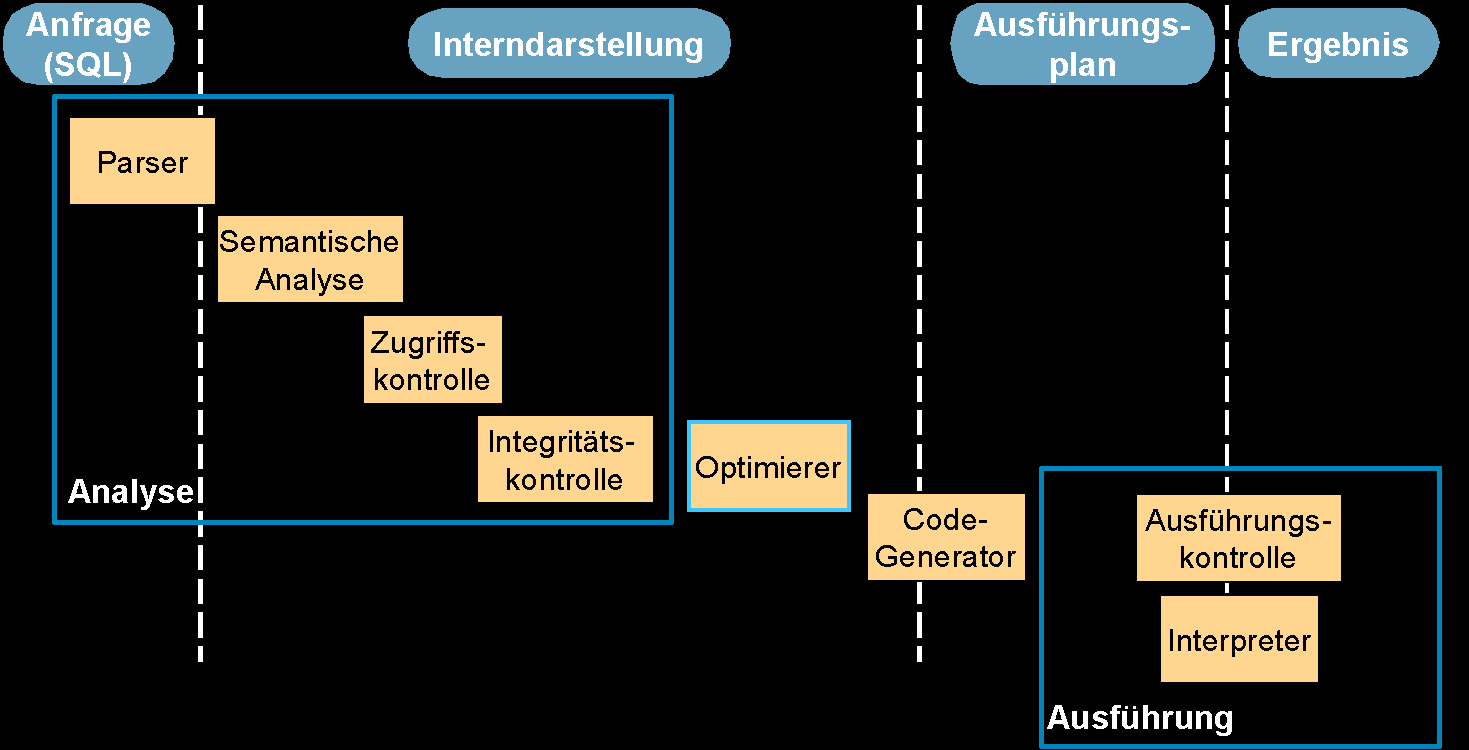
\includegraphics[width=1\linewidth]{Pictures/U10-Beamer-Anfrageverarbeitung}
\pagebreak
\end{beamerText}


\beamertxt{\pagebreak}

\section{Optimierung}

In dieser Aufgabe sollen verschiedene Implementierungsmöglichkeiten von Operatoren betrachtet und anhand ihrer Kosten verglichen werden.

\subsection*{Szenario}

Gegeben sind folgende Tabellen:

\texttt{L(\underline{l}, m[M], n[N]), m[M] NOT NULL, n[N] NOT NULL} \\
\texttt{M(\underline{m}, d, e)} \\
\texttt{N(\underline{n}, f, g)}

Folgende Attribute sind indiziert: \texttt{L.l, L.m, M.m, N.n}

Folgende Informationen sind jeweils im Systemkatalog abgelegt:

\begin{tabular}{p{2.5cm} p{10.97cm}}
	\hline
	\textbf{Bez\normaltxt[.]{eichnung}}  & \textbf{Beschreibung} \\
	\hline
	$B(S)$								& Anzahl der Blöcke, aus denen die Relation S besteht \\
	\hline
	$T(S)$								& Anzahl Tupel, die in der Relation S enthalten sind \\
	\hline
	$\mathrm{bfr}(S)$			& Mittlerer Blockungsfaktor der Relation S; ergibt sich aus $\frac{T(S)}{B(S)}$ \\
	\hline
	$V(S.a)$							& Anzahl der unterschiedlichen Werte, die für das Attribut a in S vorkommen \\
	\hline
\end{tabular}

\beamertxt{\pagebreak}

Folgende Werte sind bekannt:

$B(L) =       5.000 \\
B(M)  =       1.000 \\
B(N)  =         500 \\
T(L)  =     100.000 \\
T(M)  =      10.000 \\
T(N)  =       5.000 \\
V(N.f) =      3.000$

Vereinfachende Annahmen:
\begin{itemize}
	\item Wir betrachten nur die Kosten für Ein-/Ausgabe vom Hintergrundspeicher.
	\item Alle Indizes werden komplett im Arbeitsspeicher gehalten.
\end{itemize}

\beamertxt{\pagebreak}

\subsection*{Operatoren}

Die Kostenformeln sind aus Übungsblatt~12 bekannt:

Scan:\\
\begin{tabular}{p{3.2cm} p{5.5cm} p{4.5cm}}
  \hline
  \textbf{Impl\normaltxt[.]{ementierung}} &
  \textbf{Kosten} &
  \textbf{Einschränkungen} \\
  \hline
  TableScan (S) &
  $B(S)$ &
  \\
  \hline
  IndexScan(S) &
  $50 \cdot \left \lceil{ B(S) \cdot \mathrm{Selektivit"atsfaktor} }\right \rceil $ &
  Nur wenn geeigneter Index vorhanden (Kosten für wahlfreien Blockzugriff: 50) \\
  \hline
\end{tabular}

Join:\\
\begin{tabular}{p{3.7cm} p{4cm} p{5.5cm} }
	\hline
	\textbf{Impl\normaltxt[.]{ementierung}} 	& \textbf{Kosten}  &  \textbf{Einschränkungen}																								\\
	\hline
	NestedLoopJoin(S, T)			& $C(S) + B(S) \cdot C(T)$ 						& 																										\\
	\hline
	SortMergeJoin(S, T)				& $C(S) + C(T) + 2 \cdot (B(S) + B(T))$  	& Nur, wenn Gleichverbund  															\\
	\hline
	HashJoin(S, T) 					& $C(S) + C(T)$ 											& Nur, wenn Gleichverbund und eine Tabelle in den Puffer passt 	\\
	\hline
\end{tabular}

Weitere Operatoren:\\
\begin{tabular}{ p{3.7cm} p{4cm} p{5.5cm}}
	\hline
	\textbf{Operator} 	& \textbf{Kosten}  		&  \textbf{Bemerkungen}	\\
	\hline
	SEL(S)						& $C(S)$ 						& 										\\
	\hline
	PROJ(S)						& $C(S)$						& 										\\
	\hline
\end{tabular}

Dient die Ausgaberelation $S$ eines Operators A als Eingabe für einen weiteren Operator B, so sind die Kosten von A als $C(S)$ bereits in der Kostenformel für B enthalten.


\subsection*{Aufgaben}

\begin{enumerate}[a)]

	\item Gegeben seien Ausführungspläne für das folgende SQL-Statement.
	Bestimmen Sie jeweils die Ausführungskosten.

	\begin{lstlisting}
SELECT *
FROM   L JOIN M ON (L.m = M.m)
WHERE  L.l = 1000;
	\end{lstlisting}

	\begin{enumerate}[i)]

\item
Ausführungsplan 1:

	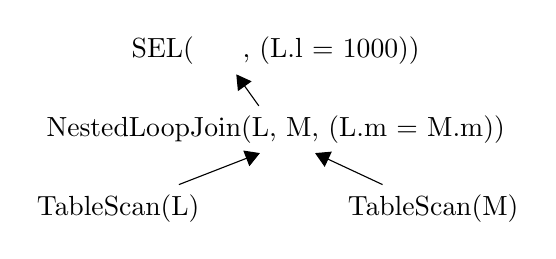
\begin{tikzpicture}
		\node (sel) at (0,0) {SEL( \hspace{0.5cm}, (L.l = 1000))};
		\node  (nested_loop) [below of = sel] {NestedLoopJoin(L, M, (L.m = M.m))};
		\node (L) [below of = nested_loop, xshift=-2cm] {TableScan(L)};
		\node (M) [below of = nested_loop, xshift=2cm] {TableScan(M)};
		\draw[-triangle 60] (L) -- ($(nested_loop.south) + (-0.2,0)$);
		\draw[-triangle 60] (M) -- ($(nested_loop.south) + (0.5,0)$);
		\draw[-triangle 60] (nested_loop) -- ($(sel.south) + (-0.5,0)$);
	\end{tikzpicture}

\begin{solution}
Der Nested-Loop-Join ist, bei den in dieser Aufgabe angesetzten Kostenformeln, der einzige nicht symmetrische Operator, d.\,h.\ für den Nested-Loop-Join ergeben sich unterschiedliche Kosten für Nested-Loop-Join(A, B) und Nested-Loop-Join(B, A).
Exemplarisch wird in dieser Aufgabe die Berechnung beider Varianten gezeigt, im Folgenden jedoch nur noch die kostengünstigere Variante betrachtet.

	\textbf{Ausführungsplan 1:}
	\begin{align*}
		\mathtt{TableScan}(L)         & = B(L) = 5.000                                                         \\
		\mathtt{TableScan}(M)         & = B(M) = 1.000                                                         \\
		\mathtt{NestedLoopJoin}(L, M) & = C(L) + B(L) \cdot C(M) =                                             \\
		                              & =\mathtt{TableScan}(L)+ B(L) \cdot \mathtt{TableScan}(M) =  5.005.000  \\
		\mathtt{NestedLoopJoin}(M, L) & = C(M) + B(M) \cdot C(L) =                                             \\
		                              & = \mathtt{TableScan}(M) + B(M) \cdot \mathtt{TableScan}(L) = 5.001.000
	\end{align*}
	$\Rightarrow$ Kosten: $5.001.000$ \\
	\end{solution}

	\begin{note}
	Für die Selektion fallen keine weiteren Kosten mehr an -- siehe Aufgabenstellung.
	\end{note}

\item
Ausführungsplan 2:

	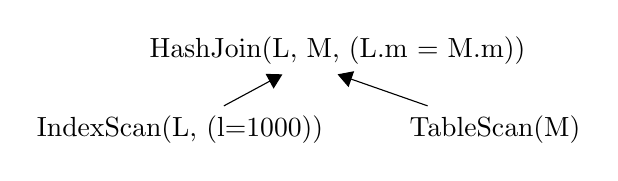
\begin{tikzpicture}
		\node (join) at (0,0) {HashJoin(L, M, (L.m = M.m))};
		\node (L) [below of = join, xshift=-2cm] {IndexScan(L, (l=1000))};
		\node (M) [below of = join, xshift=2cm] {TableScan(M)};
		\draw[-triangle 60] (L) -- ($(join.south) + (-0.7,0)$);
		\draw[-triangle 60] (M) -- (join.south);
	\end{tikzpicture}

	\begin{solution}
	\textbf{Ausführungsplan 2:}
	\begin{align*}
		\mathtt{IndexScan}(L)  & = 50                                                                 \\
		                       & \text{L.l ist PK, daher liefert er nur ein Tupel und der}           \\
		                       & \text{Selektivitätsfaktor ist $\frac{1}{T(L)} = \frac{1}{100000}$} \\
		\mathtt{TableScan}(M)  & = 1.000                                                              \\
		\mathtt{HashJoin}(L,M) & = C(L) + C(M) = \mathtt{IndesScan}(L) + \mathtt{TableScan}(M) =      \\
		                       & =  50 + 1000
	\end{align*}
	$\Rightarrow$ Kosten: $1.050$

	Auch für ein Tupel muss man einen ganzen Block lesen.
	Für das wahlfreie Lesen eines Blocks fallen nach den gegebenen Formeln Kosten von 50 an.

	\textbf{Erkenntnis:} Kleine Änderungen können unglaubliche Ergebnisse erzielen.
	\end{solution}

\item
Ausführungsplan 3:\deepen

\cprotEnv
\begin{normalText}
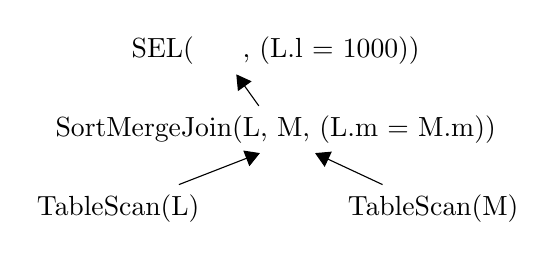
\begin{tikzpicture}
		\node (sel) at (0,0) {SEL( \hspace{0.5cm}, (L.l = 1000))};
		\node  (sort_merge) [below of = sel] {SortMergeJoin(L, M, (L.m = M.m))};
		\node (L) [below of = sort_merge, xshift=-2cm] {TableScan(L)};
		\node (M) [below of = sort_merge, xshift=2cm] {TableScan(M)};
		\draw[-triangle 60] (L) -- ($(sort_merge.south) + (-0.2,0)$);
		\draw[-triangle 60] (M) -- ($(sort_merge.south) + (0.5,0)$);
		\draw[-triangle 60] (sort_merge) -- ($(sel.south) + (-0.5,0)$);
	\end{tikzpicture}
\end{normalText}

\begin{note}
\textbf{Ausführungsplan 3:}

	$\mathtt{SortMergeJoin}(L,M) = C(L) + C(M) + 2(B(L) + B(M))$ \\
	$C(L) = \mathtt{TableScan}(L) = 5.000$  \\
	$C(M) = \mathtt{TableScan}(M) = 1.000$ \\
	$\Rightarrow$ Kosten: $18.000$
\end{note}

\item
Ausführungsplan 4:\deepen

\cprotEnv
\begin{normalText}
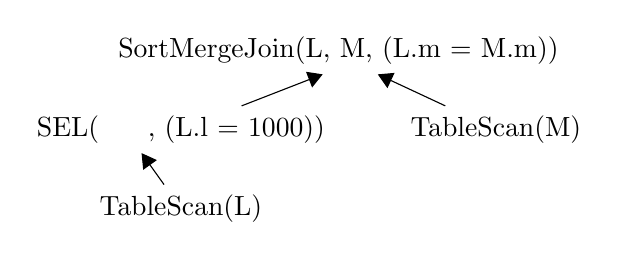
\begin{tikzpicture}
		\node  (sort_merge)  at (0,0) {SortMergeJoin(L, M, (L.m = M.m))};
		\node (sel) [below of=sort_merge, xshift=-2cm] {SEL( \hspace{0.5cm}, (L.l = 1000))};
		\node (L) [below of = sel] {TableScan(L)};
		\node (M) [below of = sort_merge, xshift=2cm] {TableScan(M)};
		\draw[-triangle 60] (sel) -- ($(sort_merge.south) + (-0.2,0)$);
		\draw[-triangle 60] (M) -- ($(sort_merge.south) + (0.5,0)$);
		\draw[-triangle 60] (L) -- ($(sel.south) + (-0.5,0)$);
	\end{tikzpicture}
\end{normalText}

\begin{note}
\textbf{Ausführungsplan 4:}

	$\mathtt{SortMergeJoin}(L,M) = C(L) + C(M) + 2(B(L) + B(M))$ \\
	$C(L) = \mathtt{TableScan}(L) = 5.000$  \\
	$C(M) = \mathtt{TableScan}(M) = 1.000$ \\
	$B(M) = 1.000$\\
	$B(L) = 1$\\
	$\Rightarrow$ Kosten: $8.002$
\end{note}

\end{enumerate}
\beamertxt{\pagebreak}

	\item Wählen Sie für die folgenden logischen Ausführungspläne passende Planoperatoren und Ausführungsreihenfolgen aus.
Gehen Sie davon aus, dass 700 Kacheln Hauptspeicher zur Verfügung stehen.
Eine Kachel sei dabei gerade so groß wie eine Seite.

Um die Zahl der möglichen Varianten in Grenzen zu halten, können Sie für die Relationen, die in die JOINS einfließen, auf die Berücksichtigung von Index-Scans verzichten und nur Table-Scans einsetzen.

	\begin{enumerate}[i)]

		\item \label{Optimierung2_1} Gegeben sind das folgende SQL-Statement und der zugehörige logische Aus"-füh"-rungs"-plan.

		\begin{minipage}{5.5cm}
		\begin{lstlisting}
SELECT *
FROM   L, M, N
WHERE  L.m = M.m
       AND L.n = N.n;
		\end{lstlisting}
		\end{minipage}
		\begin{minipage}{7cm}
		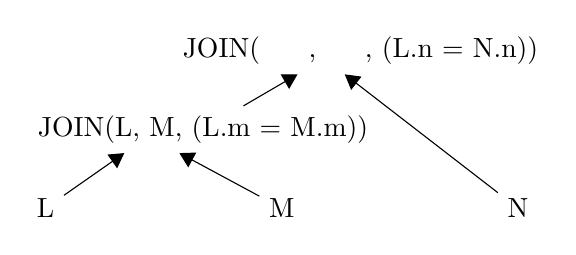
\begin{tikzpicture}
			\node (join1) at (0,0) {JOIN( \hspace{0.5cm}, \hspace{0.5cm}, (L.n = N.n))};
			\node (join2) [below of =join1, xshift=-2cm] {JOIN(L, M, (L.m = M.m))};
			\node (L) [below of = join2, xshift=-2cm] {L};
			\node (M) [below of =join2, xshift=1cm] {M};
			\node (N) [below of = join2, xshift=4cm] {N};
			\draw[-triangle 60] (join2) -- ($(join1.south) + (-0.8,0)$);
			\draw[-triangle 60] (L) -- ($(join2.south) + (-1,0)$);
			\draw[-triangle 60] (M) -- ($(join2.south) + (-0.3,0)$);
			\draw[-triangle 60] (N) -- ($(join1.south) + (-0.2,0)$);
		\end{tikzpicture}
		\end{minipage}

\begin{solution}
		Ohne Verwendung von Index-Scans sind unsere Optionen die drei verschiedenen Join-Implementierungen und die beiden möglichen Reihenfolgen der Joins.
		Das gibt schon $3 \cdot 2 = 6$ Möglichkeiten.
		Dazu kann man sparen, wenn man Zwischenergebnisse speichert.
		(Zuerst M mit N zu joinen funktioniert nicht, da sie keine gemeinsamen Attribute haben.
		Auch ein Kreuzprodukt von M und N ergibt aufgrund der Größe und den Erzeugungskosten des Zwischenergebnisses keinen Sinn.)
		\nt{$10K \cdot 5K = 50Mio$ Tupel, benötigen ca 10Mio Blöcke, Kosten vgl. NLJoin $5k \cdot 10k + 5k \approx 50M$}

		\paragraph{\color{solutioncolor}Reihenfolge: \texttt{JOIN(JOIN(L, M), N)}}

		\begin{enumerate}[1.]

			\item \texttt{JOIN(L, M)}
			  \begin{itemize}
				  \item Gleichverbund erlaubt SortMergeJoin.
				  \item HashJoin ist nicht möglich, da keine Relation in den Speicher passt.
			  \end{itemize}
			  \texttt{NestedLoopJoin(M, L):} $1.000 + (1.000 \cdot 5.000) = 5.001.000$ \\
			  \texttt{SortMergeJoin(L, M):} $5.000 + 1.000 + 2 \cdot (5.000 + 1.000) = \underline{18.000}$ \\

			  \textbf{Abschätzung der Zwischenergebnisgrößen -- Variante 1:}

			  \texttt{L.m} und \texttt{L.n} sind Fremdschlüssel, \texttt{M.m} und \texttt{N.n} Primärschlüssel und damit \texttt{UNIQUE}.
			  Damit hat jedes Tupel in \texttt{L} beim Gleichverbund höchstens einen Partner.
			  Da \texttt{L.m} und \texttt{L.n} außerdem \texttt{NOT NULL} sind, hat jedes Tupel in \texttt{L} beim Gleichverbund genau einen Partner.
			  Die Anzahl der Ergebnistupel ist damit $T(L)=100.000$.

			  Die Größe eines Tupels ist die Summe der Einzelgrößen: \\
			  $\mathrm{bfr}(L) = 20$, $\mathrm{bfr}(M)= \mathrm{bfr}(N) = 10$

			  $\Rightarrow \mathrm{bfr}(\texttt{JOIN(L, M)}) = \mathrm{bfr}(\texttt{JOIN(L, N)})= \frac{1}{0.05 + 0.1} = \lfloor6,67\rfloor = 6$ (der Rest ist Verschnitt).
			  Das bedeutet $100.000$ Tupel benötigen $16.667$ Blöcke!

			  Diese Abschätzung geht davon aus, dass alle Blöcke bis auf den Verschnitt komplett mit Tupeln gefüllt sind.
			  Bei variabel langen Sätzen wird die Satzlänge als statistisch unabhängig vom Join-Prädikat angenommen, so dass der durchschnittliche Blockungsfaktor auch für die am Join beteiligten Sätze repräsentativ ist.
			  Außerdem wird der Effekt vernachlässigt, dass nach dem Join weniger Verschnitt auftreten kann als vorher.

			  \textbf{Abschätzung der Zwischenergebnisgrößen -- Variante 2:}

			  Bei \texttt{JOIN(L, M)} hat jedes Tupel aus \texttt{M} im Mittel 10 Partner.
			  \texttt{B(JOIN(L, M))} ist daher $5000+10 \cdot 1000 = 15.000$ (jedes Tupel aus \texttt{L} kommt 1x, jedes aus \texttt{M} 10x vor).

			  Bei \texttt{JOIN(L, N)} hat jedes Tupel aus \texttt{N} im Mittel 20 Partner.
			  \texttt{B(JOIN(L,N))} ist daher $5000+20 \cdot 500 = 15.000$.

			  Wir verwenden die Werte aus Variante 1.
			  Variante 2 wäre aber genauso zulässig.

			\item \texttt{JOIN(JOIN(L, M), N)}
			  \begin{itemize}
				  \item Wir verwenden das günstigste Zwischenergebnis aus dem ersten JOIN.
				  \item Relation \texttt{N} passt in den Speicher, deshalb ist ein HashJoin möglich.
			  \end{itemize}

			  \texttt{NestedLoopJoin((L, M), N):} $18.000 + 16667 \cdot 500 = 8.351.500$ \\
			  \texttt{SortMergeJoin((L, M), N):} $18.000 + 500 + 2 \cdot (16.667 + 500) = 52.834$ \\
			  \texttt{HashJoin((L, M), N):} $18.000 + 500 = \underline{18.500}$ \\

		\end{enumerate}

		Hier kann man sich natürlich die Frage stellen, ob die beiden Joins für das Pipelining gleichzeitig in den Hauptspeicher passen, genauer, ob der letzte Schritt des Sort-Merge-Joins Zeitgleich zum Hash-Join ausgeführt werden kann.
		Dem Sort-Merge-Join steht zu Beginn der gesamte Arbeitsspeicher zur Verfügung, weswegen er die Relation L in $\lceil 1000/700\rceil = 2$, die Relation M in $\lceil 5000 / 700 \rceil = 8$ Teillisten auf, welche einzeln sortiert auf dem Laufwerk gespeichert werden.
		Im letzten Schritt wird nun von jeder dieser Teillisten ein Block geladen, das passende Tupel generiert und an den Hash-Join weitergeleitet.
		Damit werden 10 (+1 für das Tupel selber) Kacheln benötigt.
		Relation L benötigt 500 Kacheln im Hauptspeicher für die Hash-Tabelle, es stehen $700-11=689$ zur Verfügung.
		Das reicht aus.

		\paragraph{\color{solutioncolor}Reihenfolge: \texttt{JOIN(JOIN(L, N), M)}}

		\begin{enumerate}[1.]

			\item \texttt{JOIN(L, N)}

			  \texttt{NestedLoop(N, L):} $500 + (500 \cdot 5.000) = 2.500.500$ \\
			  \texttt{SortMerge(L, N):} $5.000 + 500 + 2 \cdot (5.000 + 500) = 16.500$ \\
			  \texttt{HashJoin(L, N):} $5.000 + 500 = \underline{5.500}$ \\

			\item \texttt{JOIN(JOIN(L, N), M)}

			  \texttt{NestedLoop(M, (L, N)):} $1.000 + (1.000 \cdot 5.500) = 5.501.000$ \\
			  \texttt{SortMerge((L, N), M):}  $5.500 + 1.000 + 2 \cdot (16.667 + 1.000) = \underline{41.834}$ \\
			\texttt{HashJoin((L, N), M):} Nicht möglich, da Zwischenergebnis zu groß.

		\end{enumerate}

\end{solution}

		\item Gegeben sind das folgende SQL-Statement und der zugehörige logische Aus"-füh"-rungs"-plan.

		\begin{minipage}{5.5cm}
		\begin{lstlisting}
SELECT *
FROM   L, M, N
WHERE  L.m > M.m
       AND L.n = N.n;
		\end{lstlisting}
		\end{minipage}
		\begin{minipage}{7cm}
		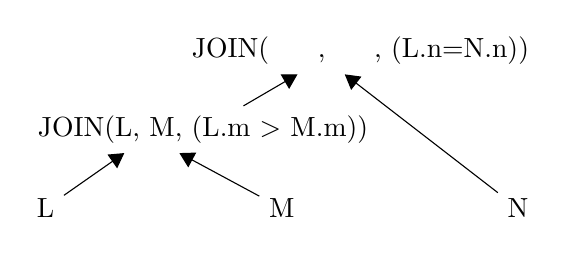
\begin{tikzpicture}
			\node (join1) at (0,0) {JOIN( \hspace{0.5cm}, \hspace{0.5cm}, (L.n=N.n))};
			\node (join2) [below of =join1, xshift=-2cm] {JOIN(L, M, (L.m $>$ M.m))};
			\node (L) [below of = join2, xshift=-2cm] {L};
			\node (M) [below of =join2, xshift=1cm] {M};
			\node (N) [below of = join2, xshift=4cm] {N};
			\draw[-triangle 60] (join2) -- ($(join1.south) + (-0.8,0)$);
			\draw[-triangle 60] (L) -- ($(join2.south) + (-1,0)$);
			\draw[-triangle 60] (M) -- ($(join2.south) + (-0.3,0)$);
			\draw[-triangle 60] (N) -- ($(join1.south) + (-0.2,0)$);
		\end{tikzpicture}
		\end{minipage}

		\begin{solution}
		Unsere Optionen bleiben im Prinzip gleich.
		Allerdings beherrscht nur der Nested-Loop-Join etwas anderes als den Gleichverbund.

		\paragraph{\color{solutioncolor}Reihenfolge: \texttt{JOIN(JOIN(L, M), N)}}

		\begin{enumerate}[1.]

			\item \texttt{JOIN(L, M)}

			  \texttt{NestedLoopJoin(M, L):} $1.000 + (1.000 \cdot 5.000) = \underline{5.001.000}$

			  \textbf{Abschätzung der Zwischenergebnisgrößen:}

			  Bei \texttt{JOIN(L, M)} wird jedes Tupel aus L mit im Mittel $\frac{T(M)}{2} =5.000$ Tupeln aus M gejoint (oder umgekehrt).\\
			  Die Anzahl der Tupel ist daher $\frac{T(L) \cdot T(M)}{2}=500.000.000$.\\
			  Die Größe eines Tupels ist die Summe der Einzelgrößen:\\
			  $bfr(L) = 20\Rightarrow \frac{1}{20}$~[Blöcke], $bfr(M) = 10\Rightarrow \frac{1}{10}$ [Blöcke].\\
			  Tupelgröße: $\frac{1}{10}+\frac{1}{20} = \frac{3}{20}$ [Blöcke].\\
			  $\Rightarrow bfr(\texttt{JOIN(L, M)}) = \left\lfloor\frac{1}{\frac{3}{20}}\right\rfloor = \left\lfloor \frac{20}{3}\right\rfloor =  \lfloor6,67\rfloor = 6$.
			  Damit hat das Zwischenergebnis von \texttt{B(JOIN(L, M))} 83.333.334 Blöcke.

			  Der Abschätzung liegen die gleichen Annahmen zugrunde wie Variante 1 in Teilaufgabe \ref{Optimierung2_1}).

			  Für \texttt{JOIN(L, N)} gilt das oben in Teilaufgabe \ref{Optimierung2_1}) ermittelte Ergebnis (16.667 Blöcke).

			\item \texttt{JOIN(JOIN(M, L), N)}

			  \texttt{NestedLoopJoin((M, L), N):} $5.001.000 + (83.333.334 \cdot 500) \approx 42$ Milliarden
			  \texttt{NestedLoopJoin(N, (M, L)):} $500 + (500 \cdot 5.001.000) = 2.500.500.500 42 \approx 2,5$ Milliarden

			\begin{note}
			(Table-Scan)

			\texttt{NestedLoopJoin((M, L), N):} $5.001.000 + (83.333.334 \cdot 50 \cdot \left \lceil{ 500 \cdot \frac{1}{5000} }\right \rceil ) \approx 4$ Milliarden (Index-Scan mit Selektivitätsfaktor $\frac{1}{T(N)}$, da Gleichverbund mit Primärschlüssel)

			Index-Scan hier nur beispielhaft als Anmerkung, da er sonst bei allen anderen Varianten auch berücksichtigt werden müsste und das die Aufgabe noch mal deutlich verlängern würde.
			\end{note}

			  \texttt{SortMergeJoin((M, L), N):} $5.001.000 + 500 + 2 \cdot (83.333.334 + 500) = 171.669.168$ \\
			  \texttt{HashJoin((M, L), N):} $5.001.000 + 500 = \underline{5.001.500}$

		\end{enumerate}

		\paragraph{\color{solutioncolor}Reihenfolge: \texttt{JOIN(JOIN(L, N), M)}}

		\begin{enumerate}[1.]

			\item \texttt{JOIN(L, N)} (wie in Teil \ref{Optimierung2_1})

			  \texttt{NestedLoopJoin(N, L):} $500 + (500 \cdot 5.000) = 2.500.500$ \\
			  \texttt{SortMergeJoin(L, N):} $5.000 +500 + 2 \cdot (5.000 + 500) = 16.500$ \\
			  \texttt{HashJoin(L, N):} $5.000 + 500 = \underline{5.500}$ \\

			\item \texttt{JOIN(JOIN(L, N), M)}

			  \texttt{NestedLoopJoin(M, (L, N)):} $1.000 + (1.000 \cdot 5.500) = \underline{5.501.000}$

		\end{enumerate}

		\textbf{Erkenntnis:} Mit den vorgegebenen Operatoren hat das Selektionsprädikat große Auswirkungen auf die Ausführungskosten.
		Beste Lösung ist 5.001.500 gegenüber 18.500 oben.
		Dabei ist der einzige Unterschied, dass im SQL-Statement "`$>$"' statt "`$=$"' steht.

		\end{solution}

	\end{enumerate}

\end{enumerate}


\end{document}
